\documentclass[11pt]{article}

\usepackage[T1]{fontenc}
\usepackage{amsmath}
\usepackage{graphicx}
\usepackage[margin=1in]{geometry}
\usepackage[font=small,labelfont=bf]{caption}

\graphicspath{{figures/}}

\title{Coarse-Grained Local Diabatic Representation}
\author{}
\date{}

\begin{document}

\maketitle

\section{SO$_2$ benchmark}

Figure~\ref{fig:so2-partitions} compares two coarse-grained electronic
partitions against full local-diabatic-representation (LDR) dynamics on the
same nuclear grid. The two-primary/one-secondary partition retains the
symmetric stretch $q_s$ and bend $\theta$ as primary coordinates and expands
the antisymmetric stretch $q_a$. The one-primary/two-secondary partition
retains only $q_s$ and expands both $(\theta,q_a)$.

\begin{figure}[!htbp]
  \centering
  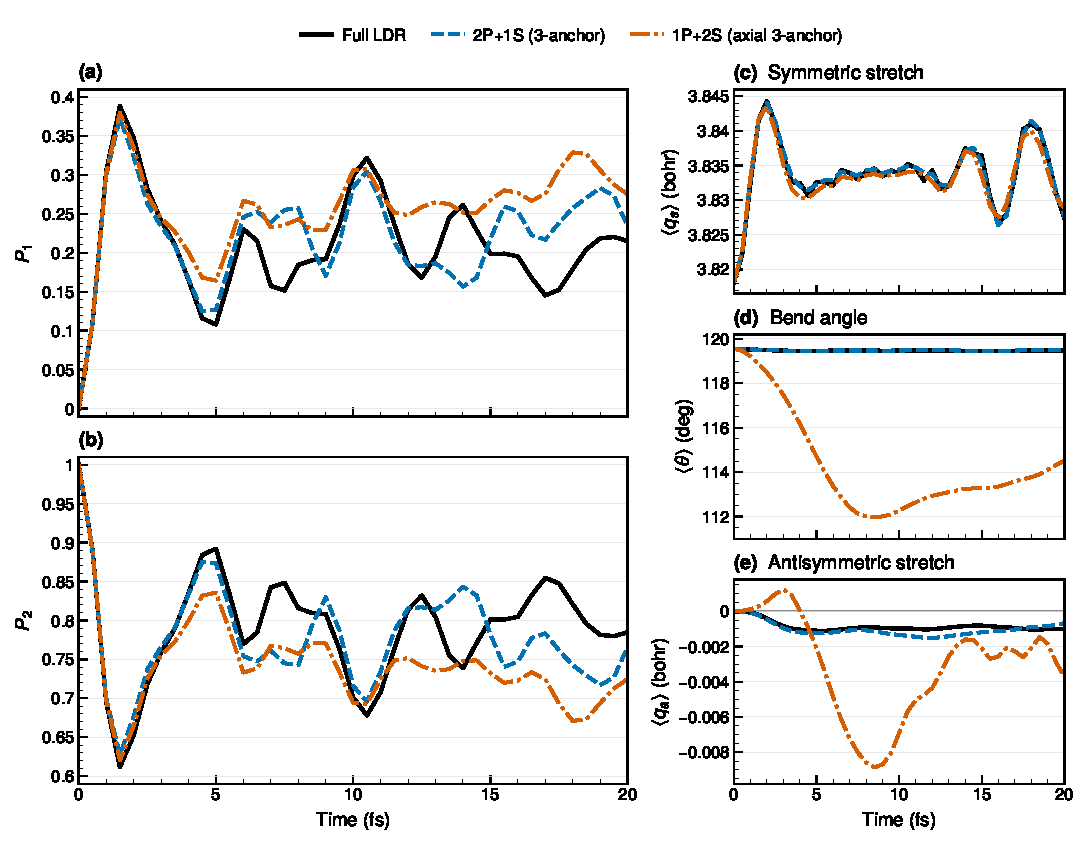
\includegraphics[width=0.9\textwidth]{so2_cgldr_partition_comparison.pdf}
  \caption{%
    Spin-pure SO$_2$ dynamics on the matched $9\times9\times9$ nuclear grid.
    The left column shows the populations $P_1$ and $P_2$ of electronic states
    $S_1$ and $S_2$; the right column shows the expectation values of the
    symmetric stretch, bend angle, and antisymmetric stretch. Full LDR is
    shown by solid black curves. The dashed blue curves are the
    two-primary/one-secondary CGLDR calculation with a three-anchor relaxed-PT
    representation along $q_a$. The dash-dotted orange curves are the axial
    one-primary/two-secondary CGLDR calculation with three anchors along each
    secondary coordinate. Keeping $\theta$ as a primary coordinate preserves
    the bend dynamics, whereas expanding $\theta$ produces a systematic bend
    displacement and larger late-time population errors.}
  \label{fig:so2-partitions}
\end{figure}

\end{document}
